\chapter{Background on Biological Collections}\label{biodiversity_data}


% Biological Collections Data
% ---------------------------
% Characteristics of occurrence data?
%  Punctual data, often obtained in an opportunistic fashion
%  May include collectors field notes.
%  Main assets of a occurrence record: taxon, location, datetime {Graham2004} -> for us, also collectors
%  Biological collections
%  Data collection is typically opportunistic.
% \cite{Hardisty2013}.

% Biological collections
Biological collections are scientific repositories where biological materials, in the form of physical specimens, are systematically deposited and preserved to be used for scientific purposes. 
Throughout this text we use the term ``biological collections'' as a synonym for \textit{Natural History Collections (NHC)}, the later being more widely adopted in biodiversity informatics literature.
Such collections are typically hosted and curated by institutions like herbaria and natural history museums, which provide appropriate physical infrastructure and human resources for ensuring both the long-term preservation of the collections and their accessibility to the scientific community.
%In addition, these institutions usually count with large networks of associated contributors, including professional collectors and taxonomists.
% Data acquisition: (1) New collecting expeditions; (2) Collections exchanges materials with other institutions

In this chapter we give an overview of how data in biological collections is structured.
We describe the semantics of species occurrence records in section \ref{section:occurrence_data}.
We also discuss some aspects regarding the quality and limitations of such data, and how we deal with these limitations.
Before delving into the characterization of biodiversity data we first review the definitions of some domain-specific terms that will be used throughout this text. 

% =====================
% Terms and Definitions
% ---------------------
\section{Biodiversity-related terms and definitions} \label{section:biodiversity_terms}

Throughout this work we use definitions from the \textit{International Code of Nomenclature for algae, fungi and plants} (ICN) \cite{McNeill2012}. This document outlines a set of rules and guidelines for scientifically naming and grouping plants, fungi and algae, consisting of a universally adopted reference by the botanical scientific community. Nomenclature best-practices for other groups of organisms are governed by other (though similar) documents.

\paragraph*{Taxonomy.}
Within the domain of biology, taxonomy is, in a general sense, the science of classification of organisms. 
Organisms are classified according to their shared characteristics using a hierarchical system, in which organisms are grouped at distinct levels of specificity (or \textit{taxonomic ranks}).
Groups of organisms that are more specific are nested within broader ones. 
For an analogy with set theory, a taxonomic classification system can be thought as being similar to a hereditary (or pure) set, in that all members in a set are, recursively, also required to be sets.

\paragraph*{Taxonomic Rank.}
The taxonomic rank of a grouping of organisms is the level of the taxonomic hierarchy at which it is defined. The most relevant ranks adopted in botany (in descending hierarchical order) are \textit{Kingdom}, \textit{Phylum} (or \textit{Division}), \textit{Class}, \textit{Order}, \textit{Family}, \textit{Genus}, \textit{Species}, as stated in \textit{Art. $3.1$} of ICN.

\paragraph*{Taxonomic Resolution.}
The taxonomic resolution of a biological sample is the taxonomic rank of the most specific taxonomic determination that has been assigned to it.
For instance, if a sample has been determined up to the level of \textit{species}, this rank is also its taxonomic resolution.
As taxa relate to each other on a tree-like hierarchical structure (with each child taxon having exactly one parent, while a parent taxon can have one or more children), taxonomic identities of a specimen at ranks higher than its resolution can be directly determined.
Although this term is not included in the ICN document, we use this definition throughout this text.

\paragraph*{Taxon.}
A taxon is a taxonomic group of organisms at the level of any rank (ICN \textit{Art.1.1}), which are considered by professional taxonomists to form a \textit{taxonomic unit}. Plural is \textbf{taxa}.

\paragraph*{Species.}
Species is one of the taxonomic ranks organisms can be determined by professional taxonomists as belonging to. It is regarded to be a basic unit of taxonomic classification, although organisms can be further classified in lower-hierarchy taxonomic ranks (infraspecific ranks).
Differently from other ranks, the name of a species is composed using a binomial nomenclature system, in which the name of the genus it belongs to is appended to a \textit{specific epithet}.
Examples of species names are \textit{Caryocar brasiliense}, \textit{Myrcia guianensis}, \textit{Solanum lycocarpum}.

\paragraph*{Specimen.}
When botanists sample organisms in field they either collect part of the organism (\textit{e.g.} a branch of a tree), the entire organism (\textit{e.g.} the entire body of a weed) or multiple individuals of the same type (\textit{e.g.} a bunch of identical, very small-sized mosses). 
Any of these collected biological materials is an evidence of the existence of a particular organism at some place and time, and should be properly deposited in a biological collection for being preserved as a reference. 
A specimen is defined as one of such evidences, and refers to a punctual observation of a single kind of organism. 
For the formal definition refer to \textit{Art. $8.2$} of ICN. 
Although a specimen could be classified by a taxonomist as being a representative of a given species, this is not a requirement for it to be included in scientific collections. Although taxonomists classify specimens in a best effort manner (the most taxonomically precise as possible), sometimes only higher ranks can be determined. The highest taxonomic rank at which the specimen could be identified is known as its \textbf{taxonomic resolution}.
After properly deposited in a biological collection, each record receives a taxonomic identification that assigns the individual to a taxonomic group (a taxon), in a best-effort manner.







% ===============
% Occurrence Data
% ---------------
\section{Species occurrence data} \label{section:occurrence_data}
Physical specimens stored in biological collections (also referred to as \textit{vouchers}) are often associated to complementary information, either annotated by the responsible collectors during the collecting act; or annotated at later stages, after the specimen is deposited in the collection \cite{Chapman2005}.
Information from the collection event include the \textit{date, time} and the \textit{geographic location} where the specimen was collected; the names of the \textit{collectors} who were involved in the collection event; and eventual \textit{field notes} describing contextual remarks, such as weather conditions, habitat features, or the sampling method used.
Other crucial piece of information is the \textit{taxonomic identity} of the specimen, determined by taxonomists after the biological material is incorporated to the collection.

The taxonomic identity of a specimen includes not only the taxon name assigned to the sample, but also its nomenclatural status and authorship, the name of the taxonomist who has identified the specimen, and other quality-related information.
As the taxonomic identity of a specimen can be re-evaluated by specialists several times after the first determination (though it requires that the investigator has access to the physical specimen), a history of determinations is usually stored in the collection.

% Occurrence data
Vouchered specimens, together with their associated data, is what scientifically testifies a punctual observation of a species by a collector, at some location and at some point in time, and is thus referred to as a \textit{species occurrence} record (Figure \ref{fig:occurrences_er}).
%
Three dimensions of occurrence data: taxonomic identity, space and time.

\begin{figure}[h!]
  	\centering
    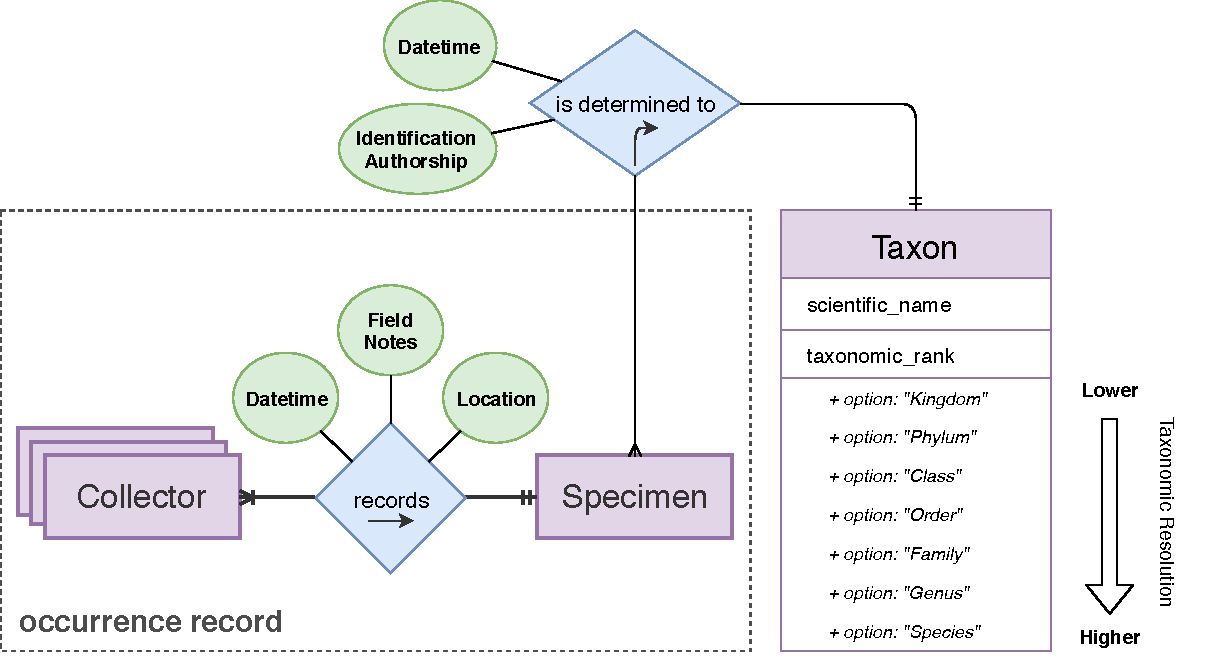
\includegraphics[width=\linewidth]{figures/collections_data/occurrences_er.pdf}
    \caption[Entity-relationship diagram illustrating the main features of occurrence records]{Entity-relationship diagram illustrating the main features of occurrence records. The cardinality of relationships is represented using the Crow's foot notation.}
    \label{fig:occurrences_er}
\end{figure}


With the development of electronic databases over the last $40$ years, many institutions have adopted computerized systems for improving the management and accessibility of specimens-related data \cite{Sunderland2013}.
However, in many regions (including Brazil and China) we face challenges on digitizing information, information is not yet digitized or integrated \cite{Meyer2016}.
% Data sharing intiatives




% Data sharing/integration
Data aggregation initiatives have addressed this limitation by facilitating data sharing and integrating many data sources (data aggregators). % data ggregators have already been mentioned
However, integration can only happen when we have data \textit{interoperability}.
Some intitiatives such as TDWG provide biodiversity informatics data standards for data integration and sharing.
DwC is the Darwin Core metadata scheme, and consists of data domains. % check Veiga2014 for refs
% TDWG first mentioned here 


%% Citizen science and informal collectors
Although biological collections have traditionally been the most traditional sources of species occurrence data, recent advances in mobile computing technology, associated to connectivity of devices to the World Wide Web, have leveraged the participation of informal groups of nature observers in recording biodiversity \cite{Silvertown2009}.
The nature of such records is similar to those from biological collections in that they are punctual observations of specimens in nature, but also have some important distinctions: (i) as nature observers usually do not collect biological materials, there are no vouchered specimens, which difficults the taxonmoic determination of the recorded specimen; (ii) taxonomic determinations result from a collaborative community, not and not by professional taxonomists. 





\section{Limitations of data}
% Presence vc presence-absence data
% Collectors Behavior (TerSteege2011)
% Newbold2010
% Limitations: sampling bias, lack of assessment of sampling effort, lack of geographic coverage

% Data issues
Although biodiversity scientists have certainly benefited from open access to massive volumes of species occurrence data from many biological collections, the availability of detailed information is still very scarce for most known organisms.
This scenario, referred to as the \textit{Wallacean Shortfall} \cite{Lomolino2004}, is even more critical for discovering and managing threatened species in megadiverse countries, which still remain largely unexplored for many regions and taxonomic groups \cite{Soberon2004}.
%
% Presence-only data
Moreover, given the non-systematic and opportunistic nature of how specimens are usually recorded, biological collections provide no reliable information on the absence of species extent of sampling effort towards each location, which makes .

has been absence of species, nor on the extent of sampling effort employed across geographic space.
The \textit{presence-only} nature of species occurrence data limits its usability for some modeling 

Moreover, the \textit{presence-only} nature of species occurrence data limits its usability for some modeling approaches, which require not only information on the existence of species in geographical space, but also on their absence.
While an occurrence record provides evidence for the existence of a species at some location, the absence of records does not mean species absence.

Nevertheless, as presence-absence data are rare and usually costly to collect, some methods have been proposed for fitting the models using pseudo-absences (or background data) derived from presence-only occurrence records \cite{Phillips2009}.

Second, while an occurrence record provides evidence for the existence of a species at some location and time, the absence of a record of a species does not testify for its absence.
Occurrence data are classified as presence-only data.
The absence of a species does not testify for its absence.
As opposed to surveys which use grid designs, species occurrences are typically gathered in an opportunistic way.
According to \citeonline{Zaniewsky2002}, there are two important limitations of presence-only data:
First, the non-systematic sampling routines which characterizes such data makes it challenging to characterize biases in the data. 
Second, sampling effort is also unknown, and thus observe a sampling bias of common vs. rare species.
Rare species tend to be more representative in such datasets.

adequate for data made available by biological collections is not always adequate for

assessing the conservation status of species in such countries



this limitation is even more problematic for threatened species, which tend to have few occurrences.

understanding on ecological requirements of the, the lack of species data limits the modeling , This limits our ability to 
As many applications of biodiversity data are based on ... the lack of adequate data impacts the quality of models, used for
This imposes serious limitations for understanding ecological and evolutionary aspects of many species, specially for the most imperiled ones. 
many applications of NHM data, especially for SDM \cite{Galante2017}, making it even harder to understand the ecological requirements of threatened species.
Consequently, we still lack data for studying ecological and evolutionary aspects of many species (and especially the most imperilled ones).

% Data quality
dealing with so many heterogeneous data sources also introduce new complexities related to data.
Data is not always adequate for investigating every aspect of natural systems.
Using inadequate data for studying specific aspects of biological diversity can lead to erroneous or misleading results \cite{Chapman2005}, and investigators must be aware of the inherent limitations of their data before formulating their questions. % Chapman in pg. 1

%($i$) the scarcity of data for many organisms in the world, which is referred to as the \textit{Wallacean Shortfall}
%($ii$) their inability to represent the \textit{absence} of species; and
%($iii$) the \textit{quality} of data, including errors and uncertainties.
Three important aspects of datasets from biological collections may limit their use for their intended applications.
% Wallacean Shortfall
First, detailed information on the geographic distribution of most organisms is very scarce, especially for the most imperiled ones. 
This scenario, referred to as the \textit{Wallacean Shortfall} \cite{Lomolino2004}, is even more critical for megadiverse countries, which still remain relatively unexplored for many taxonomic groups \cite{Soberon2004}.
The low availability of occurrence data for most species imposes serious limitations for many applications of NHM data, especially for SDM \cite{Galante2017}, making it even harder to understand the ecological requirements of threatened species.

% Presence-only





One important regards \textit{data quality}.
%
%
Data quality loss can be affected in multiple stages of its life cycle \cite{Chapman2005}, including the moment of the recording event, its preparation before it is incorporated, the taxonomic determination, data digitization, data storage and analysis.
%
Before being used, data quality must be characterized, which depends on the user needs.
Data quality assessment depends on its intended use \cite{}.
%
Users need a systematic way to both assess and manage data quality.
\citeonline{KochVeiga2017} have proposed a framework for systematically assessing requirements that make quality acceptable for each kind intended use, in the biodiversity informatics community.
%
Dimensions of data quality \cite{Veiga2014}
\citeonline{Veiga2014} have identified recurrent patterns of errors in occurrence data, among them:
domain value redundancy;
Nonatomic data values;
Inconsistent data values.
They have also proposed mechanisms for preventing the inclusion of errors and uncertainities during the data entry, as a measure for the improvement of data quality.


We have identified three important limiting aspects of biological collections. % (i) Coverage; (ii) Data quality (errors, uncertainities and biases); (iii) data biases; unavailability of absence data.
The first one concerns its \textit{coverage}. 
The ?lack of proper funding and financial support? make many megadiverse countries still relatively unexplored for many taxonomic groups \cite{Soberon2004}.
Despite their efforts towards documenting life on Earth, biological collections contain very limited information on the geographic distribution of organisms, especially for the most imperiled ones, a scenario which is referred to as the \textit{Wallacean Shortfall} \cite{Lomolino2004}.
This makes it even more difficult to understand aspects of their ecology.
% How to deal with sdm when we have few data available for species? Galante2017



This shortage of data, combined with insufficient quality limits the use of data from biological collections for many intended applications, many of which require an intensive amount of data to be available \cite{Guisan2007}.
The low availability of occurrence data for most species imposes serious limitations for many applications of NHM data, especially for SDM \cite{Galante2017}.


Besides the limitation on the availability of data, another limitation concerns its \textit{quality}.

Different data limitations for each dimension \cite{Meyer2016}.

Some of the most common problems include the wrong identification of specimens; using outdated taxonomy; bad georreferencing of records \cite{Soberon2004}.




\subsection{Errors and uncertainity}
Errors in biological collections datasets can be of distinct types, and are more common on the taxonomic identity and spatial information, and can be manually inspected by comparing with collector field notes \cite{Graham2004}.
Determination issues: many specimens are incorrectly identified;



\paragraph*{Domain value redundancy.}

\paragraph*{Data atomicity.}

\paragraph*{Consistency.}

%
\paragraph*{Taxonomic errors.}
The accuracy of taxonomic determinations depend on the expertise of the taxonomists who evaluate the specimens.
Determination issue, as many specimens are incorrectly identified;
The accuracy of the taxonomic determination depends on the expertise of the taxonomist.
if the identification of the specimen is incorrect, and can be reevaluated if the physical specimen is available.
Typographic (misspelling) errors are particularly common.
They can be dealt with during data entry, by using authority files containing accepted names 

\paragraph*{geographic errors}commonly associated to 
wrong coordinates, 
imprecise coordinates(e.g. if the coordinate was not originally recorded, and is later inferred as the centroid of a municipality or state), 
unknown datum, 
null values being interpreted as (0,0) coordinates.
%
\paragraph*{temporal errors.}
%
There are also \textit{typographic} errors, which are common for example in the taxonomic names and in other fields, such as the collector field.

\paragraph*{inconsistencies in fields.}


\subsection{Biases}
% collector bias, taxonomic bias, (geographic bias, trait bias, historical bias, seasonal bias) % Daru2017, Haripersaud2009 
Biological collections are composed of records which have been obtained by distinct people in distinct contexts, having been usually obtained in opportunistic fashion, as opposed to having random sampling designs
Occurrence records are often recorded without random sampling, leading to biases in data.
Biases are introduced in the dataset as an effect of elements that make sampling non-random, such as the detectability, the facility to access areas...
We briefly introduce 4 types of bias (although there are other types as well).
In the context of this work, collector and taxonomic biases are the most relevant.

\paragraph*{Collector bias.}
Not all collectors contribute to the same extent to biological collections.
In fact, it has been observed that, for many biological collections, a considerable percentage of records are gathered by only a small subset of very productive collectors, while the vast majority of collectors contribute with just a few records, each \cite{Daru2017,Carine2012}.
This unbalance in the representativity of collectors is what defines the \textit{collector bias} in biological collections.
As the overall taxonomic composition of collections --- as well as the geographical and temporal distribution of their records --- tend to reflect the particular interests and collecting behavior of their most representative collectors, collector bias is strongly related to other types of biases in the collection.

\paragraph*{Taxonomic bias.}
Not all taxa are quantitatively represented in biological collections in the same proportions as they occur in natural systems.
Instead, the taxonomic composition of collections reflect the interests of the communities of collectors contributing to them.
Taxonomic bias is intrinsically related to collector bias, as the overall composition of biological collections tend to reflect the interests of their most productive collectors.
The collection is biased towards taxonomic groups most sampled by the most productive collectors.
%
Rare species tend to be more overrepresented in biological collections in comparison to common species \cite{}.
%
%Some studies have proposed to assess taxonomic bias of collectors by comparing the representativity of each taxon on their sets of records to the herbarium \cite{Haripersaud2009}. %Such approaches give at most a view of how well a collector represents the composition of the collection.
%However, if we consider the herbarium itself is composed of contributions of multiple collectors each with particular interests --- and therefore also biased ---, the herbarium is biased, not representing well the natural communities.
%As it is very common that collectors towards sampling the highest number of species as possible in localities they visit, the collection is non-random, and rare species tend to be overcollected and common species, undercollected \cite{TerSteege2011}.
%Biases of the most productive collectors would be hard to assess.

\paragraph*{Geographic bias.}
% [Kadmon, R., O. Farber, and A. Danin. 2004. Effect of roadside bias on the accuracy of predictive maps produced by bioclimatic models] 
Collection sites are not randomly selected in geographic space, nor they are all sampled to the same extent.
As features of the landscape make some areas more accessible for collection activities than others \cite{Hijmans2000}, collectors tend to prioritize those to maximize their productivity while minimizing costs.
Geographic bias arises as a consequence of non-uniform collecting effort in geographic space, and tends to reflect the preferred locations of the most productive collectors.
Some regions that are more accessible being thoroughly sampled (such as areas near urban centers, roadsides and margins of rivers);
while others which are more inaccessible, such as rainforests, being only poorly or not sampled at all.
%
Also, some countries are more sampled than others.
A compilation of the representativity of plants in GBIF by \citeonline{Meyer2016} has shown that among the most representative countries and regions are the United States (mainly the west coast), Central America, countries in Europe (including the nordic countries), Australia, Japan, New Zealand.
%
Assessing patterns of species richness from species occurrence datasets has been shown to be particularly challenging due to geographical bias \cite{Hortal2007,Reddy2003}, as higher diversities of species observed in regions that are more accessible is a consequence of more intensive sampling effort.


\paragraph*{Temporal bias.}
Collection activity is not uniform over time.
Temporal bias can be further subdivided into two more specific classifications (although there are others):
Historical bias. 
Seasonal bias: Two causes: 
Biases in higher granularities, such as weekdays/weekends...


\subsection{Data completeness}
% Funk1999 Jacobs2017 Soberon2007

\subsection{Data atomicity}
Some fields in occurrence data are not atomic, which means that multiple values


\section{Improving data quality}
Although data quality can be improved by either prevention or correction, being the prevention considered more effective, as correcting the data is costly\cite{Chapman2005}, prevention is out of our scope, here we limit our scope to correction.
Here we deal with data validation and cleaning of aspects that are most relevant for the modeling we propose.
GBIF has a set of data validation routines, that base on outlier detection, that look for inconsistencies and flag them, but do not overwrite, so that they can be inspected by data user.

Data cleaning depends on the defining the intended use of data (data fit for use).

In the scope of this work, we primarily deal with the entity-resolution problem.

\subsection{The entity-resolution problem}
\citeonline{EstevaoDaSilva2016} has proposed a data mining methodology based on association rules analysis for identifying possible name variants.
\cite{Bhattacharya2007}

% Data Aggregators
Gbif provides a data preprocessing routine % https://www.gbif.org/infrastructure/processing





%% As it is common practice for botanists to record each species once during field work, some important ecological attributes such as the species abundance are not to be directly inferred from such data. {check van Gemerden 2005, from Haripersaud2009}


% Biological collections are composed of aggregates of multiple biodiversity surveys, each recorded with particular methodologies
% Records sampled using distinct methodologies can be combined for optimizing data use \cite{VanGemerden2005}.











% ============
% Data quality
% ------------
% [Soberon2004]

% Data quality among collection records is uneven -> worse for large datasets and for datasets composed by multiple sources
% Procedures are needed for correcting problems

% Quality issues: 
%% Determination issues: many specimens are incorrectly identified;
%% outdated taxonomy;
%% georreferencing errors.

% Data atomicity issues:
% Some fields are not atomic: more than one entity is represented as a single data element. 
% In the recordedBy field, Darwin Core standards state that distinct names should be separated by | (delimiter).
% This varies depending on the standard a collection uses. For example, the BRAHMS system recommends using a ';' as the delimiter.
% BRAHMS docs: https://herbaria.plants.ox.ac.uk/bol/brahms/support/documentation

% Identity issues:
% Entities are not guaranteed to have the same ids through distinct datasets.
% Even in the same datasets there may be variations in their names
% this is specially problematic for fields like the collectors field, which is overlooked for most applications of such data. 
% Some standards provide guidelines for including collectors names: last name + first initials...
% However different standards give distinct guidelines and thus name variants are common.
% How to map all name variants to the same entity? -> This leads to the Entity-resolution problem
Some common issues are: (i) including only the name of the first author of the occurrence, and eventually et.al grouping all other collectors;
(ii) format inconsistences when including multiple collectors. Some datasets do not use unique delimiter characters for separating collectors names, and thus affects the process of names atomization.
(iii) As collectors names are usually included in the form of last name followed by first initials, there are many cases of homonymous, especially for very common surnames (e.g. silva, souza,...).
There are also heteronymous, when distinct names variants are assigned to the same person. It can happen that two people have the same last name and their initials are the same (e.g. André Machado Souza or Ana Maria Souza leads to A.M.Souza).
This can also be the result of typos (e.g. souza becoming souza), or simply omiting parts of the name (e.g. if there are two collectors, A.M.Souza and A.P.Souza, omitting the middle initial makes their names indistinguishable).

% Data fit for use

In order to make data fit for its intended use the analyst must perform data cleaning.

% =============
% Data cleaning
% -------------
%[Chapman2005a]

% Why do we need data cleaning? -> We must make data fit for its indended use

% Goal: improving data quality, removing or treating entries that are 

% Adopting standardized collectors names
% Checking collectors itineraries -> look for the spatial pattern of records by the collector


% ================
% References
% ----------------
%% Museum-based informatics{Graham2004}









% Data Quality

% Preparing data 
% Data Selection
% Data Cleaning


% The Entity Resolution problem


% Homonymous names, heteronymous names
% Typographic errors
First, using different naming conventions or occasionally including typographic errors while entering the data in the database leads to multiple variants of name.
Examples of typographic errors are mis
(such as names with typographic errors) homonymous names (a name
